\documentclass[a4paper,fleqn]{tufte-handout} 
\usepackage{graphicx}

\title{Computational experiments in Science : herding horses on a daily basis}

\author{Mathieu Lagrange and Mathias Rossignol}

\begin{document}

\maketitle

\section{Introduction}

Dealing with large amount of numerical data and complex processes is the chance or the curse of many fields in science. Contrary to pure engineering approaches where the main objective is the performance, the main of science is, by experimental demonstration, to confirm or reject assumptions that have been formulated theoretically. 

Thus, those two approaches have in common the need to perform some kind of experiment which in most cases resort to 1) take data from measurements, 2) process it using algorithms built upon some assumptions about the underlying process that generated the data, 3) study if those algorithms are able to produce corresponding data that, in the engineering scenario, tentatively serves some useful purpose and in the science one, potentially validates the theory.


\section{Horses are where complexity is}

\begin{marginfigure}
\begin{center}
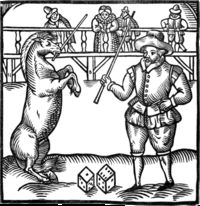
\includegraphics[width=\textwidth]{figures/hans} 
\end{center}
\caption{\label{fig:explanes} Hans is clever, but not quite: \url{https://en.wikipedia.org/wiki/Clever_Hans}}
\end{marginfigure}

Data under evaluation in today's challenges are highly multidimensional in many ways: number of dimensions, number of items, number of classes ... Fully understanding the complexity behind is an utopia rather than an achievable goal and as such every conclusion that are drawn are to be considered with care.

Among many, an issue that arises is the fact that, even if the underlying assumption that helped us to build a processing chain is correct, the implemented machine is in fact using other means to achieve the good results we are striving for. This as been coined as a "horse". More precisely, a "horse" is a system appearing capable of a remarkable human feat, e.g., music genre recognition from an audio signal, but actually working by using irrelevant characteristics (confounds) \cite{6847693}.

Adopting a purely engineering approach leaves us with the freedom to live with horses without too much concerns as only the end performance counts. As far as the performing conditions do not changes, the performance should remain unchanged. On contrary, science is not supposed to "ride" horses as engineering approaches can as it may lead to an erroneous validation of a given theory or assumption.

That being said, given the complexity researchers now daily tackle, only care, rigor, doubt and freedom of investigation, which are the cornerstones of the scientific method can help in that matter.

\section{Spotting a horse}

When tackling the issue of modeling acoustic scenes, the use of the Bag-Of-Frames (BOF) approach as proposed in \cite{aucouturier2007bag} is often considered.

However, as described in \cite{lagrange:hal-01082501}, this very good performance of the presented system is in fact due to a thankful organization of the dataset with very low intra-class diversity. The system, evaluated on datasets with higher intra-class diversity completely fails. A second outcome of the study is that the statistical model composed of mixture of Gaussians considered do not perform better than a simple averaging of the features.

\section{Herding horses}

Acknowledging the fact that most of the algorithms we build are probably horses to a certain degree, we designed some open-source tools that help us being in better control while numerical experiments.

\subsection{Data}

\begin{marginfigure}
\begin{center}
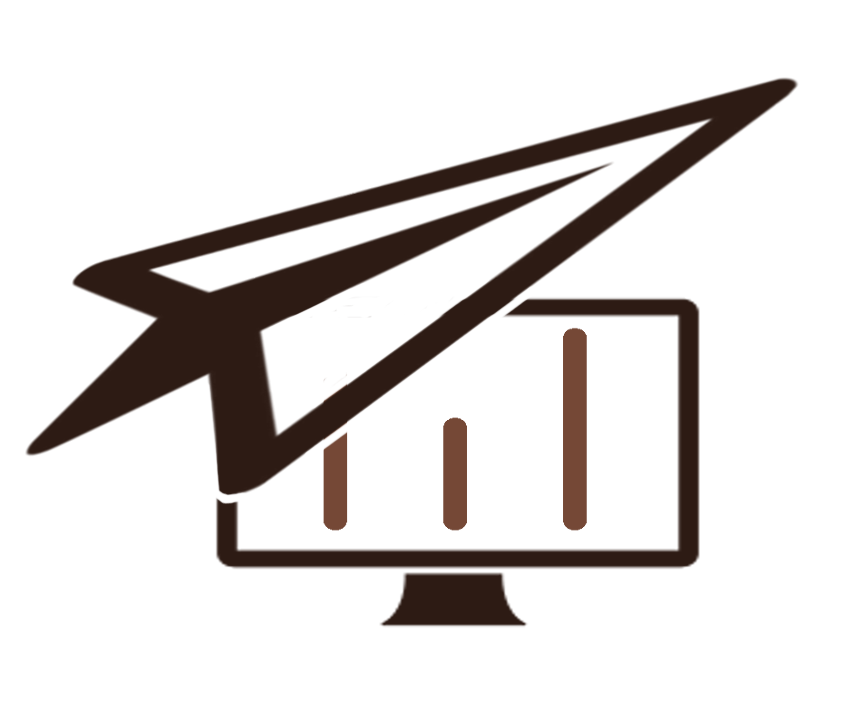
\includegraphics[width=\textwidth]{figures/logo} 
\end{center}
\caption{\label{fig:simScene} SimScene is an open source tool: \url{https://bitbucket.org/mlagrange/simscene}}
\end{marginfigure}

Algorithms perform on data, therefore the kind of data given is crucial. In our opinion, we shall
\begin{enumerate}
\item carefully craft evaluation datasets (big is not enough)
\item increase the complexity progressively with controlled data
\item share data
\end{enumerate}

In the case of acoustic scene analysis, we built a tool called \textsf{simScene} that greatly ease this process by simulating acoustic scenes with a large level of control over the morphology of the scene.%, see Figure \ref{fig:simScene}.

\subsection{Experimentation}

\begin{marginfigure}
\begin{center}
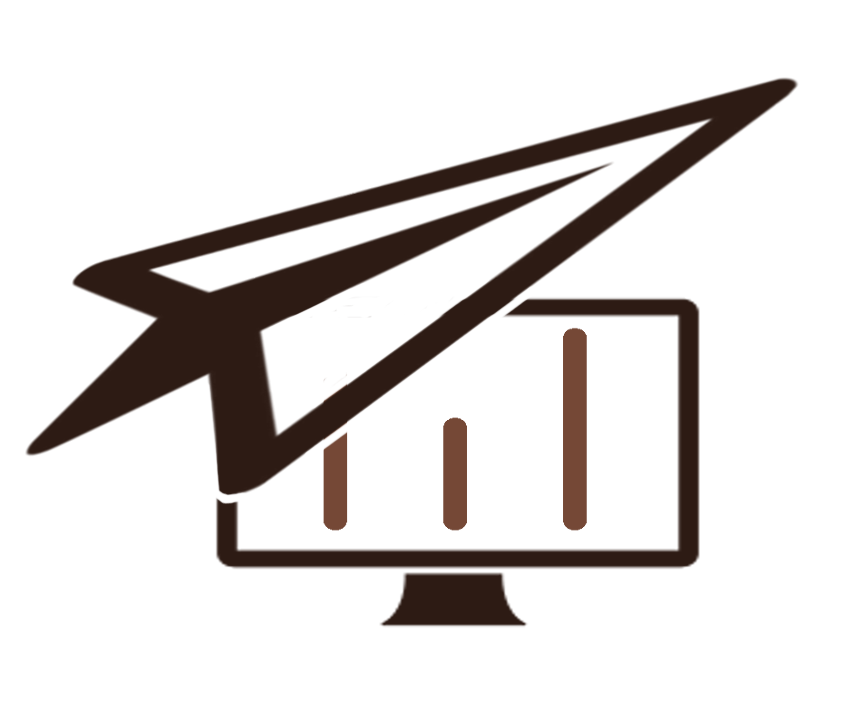
\includegraphics[width=\textwidth]{figures/logo} 
\end{center}
\caption{\label{fig:explanes} ExpLanes is an open source tool: \url{http://mathieulagrange.github.io/expLanes}}
\end{marginfigure}

Algorithms are as complex as the data they process and measuring their performance is not trivial. Therefore, in our opinion, we shall:
\begin{enumerate}
\item implement lower bounds and upper bounds baselines
\item enforce reproducibility
\item share code
\end{enumerate}

With those aims in mind, we built a tool called \textsf{expLanes} that greatly ease this process, by proposing a complete evaluation framework that strictly follows the scientific method.%, see Figure \ref{fig:explanes}.




  
\bibliographystyle{abbrvnat} 
\nobibliography{bib} 
  
\end{document}